
\section{Computational considerations}

HDG methods offer several well-known advantages over standard DG-FEM methods. 
In addition to favorable convergence properties, hybridization of the system by introducing the space \todo{Mph} can lead to a substantial reduction in globally-coupled degrees of freedom as compared to classical DG methods.
However, the complexities associated with the static condensation procedure introduce a set of non-typical computational performance considerations as compared to other high-order methods.
In this section, we provide a brief discussion of practical computational considerations specific to HDG schemes in the context of parallelization and matrix-free solvers. These topics are often overlooked or unaddressed in the literature (to DG/HDG etc ref).

A commonly cited performance advantage of HDG is the embarrassingly parallel nature of the assembly as well as the local reconstruction of the numerical solution QH UH from the trace quantity UHAT.
Means that people brush this step off computationally, as a parallel implementation should make it trivial.
However there's more to the story than that.



though it may seem counterintuitive, multi-threaded programs can sometimes run slower than their single-threaded or serial counterparts due to several reasons:

Overhead: Threads require resources for creation, termination, and synchronization. The overhead of managing multiple threads can slow down the program, especially if the computation performed by each thread is not significant compared to this overhead.
Contention: When multiple threads try to access a shared resource simultaneously, contention can occur. This could lead to a situation called a lock, where one thread has to wait for another to release a resource. In extreme cases, this can lead to a slowdown known as lock contention, where the threads spend more time waiting to access the resource than doing useful work.
False sharing: Even if different threads are working on different data, if that data is close enough in memory (i.e., in the same cache line), then the hardware can treat it as if it were shared. When one thread updates its data, the hardware will think the entire cache line has been modified and will have to update it across all the cores, leading to a significant slowdown. This is known as false sharing.
Load imbalance: If the work is not evenly distributed across threads, some threads may finish their work early and sit idle, while others are still working. This is known as load imbalance. It can result in the execution time of the program being dominated by the slowest thread.
Non-parallelizable tasks: Some tasks simply can't be parallelized effectively due to their nature, they are inherently serial (or "sequential"). This principle is encapsulated by Amdahl's Law, which states that the maximum improvement to a system's performance is limited by the portion of the system that can't be parallelized.
Memory limits: Every thread created uses some memory for its stack. If the number of threads is too high, it can cause significant memory usage, potentially leading to swapping if the system runs out of physical memory, which can drastically decrease performance.
It's worth noting that developing an efficient multi-threaded program requires careful design to minimize these issues. This can involve techniques such as fine-tuning the number of threads, avoiding contention and false sharing, balancing the load properly, and choosing appropriate data structures and synchronization primitives. But even with all these considerations, there's no guarantee that a multi-threaded solution will always outperform a well-optimized single-threaded one. It highly depends on the nature of the problem and the specific hardware the software is running on.

\section{Numerical experiments}
\label{sec:numerical_experiments}

\subsection{Implementation}%
\label{sec:implementation_details}

The finite element forward models were implemented in \texttt{C++} and make use of the finite element library \texttt{deal.ii} \cite{dealII93}.

\todo{
All surface and volume integral operators are discretized with Gaussian quadrature using $p_{\text{order}}+1$ one-dimensional (1D) quadrature points in each spatial direction, where $p_{\text{order}}$ is the polynomial order of the finite element space (space)}. 
%$W_h^\porder$.

Convergence results are reported using the relative $L^2$-errors 
\begin{equation}
  \erroru(t) = \frac{ \left\lVert \vel(\bm{x}, t) - \velh(\bm{x}, t)\right\rVert_{\LII(\dom_h)} }{ \left\lVert \vel(\bm{x}, t) \right\rVert_{\LII(\dom_h)} }, \qquad 
  \errorp(t) =\frac{ \left\lVert \p(\bm{x}, t) - \ph(\bm{x}, t)\right\rVert_{\LII(\dom_h)} }{ \left\lVert \p(\bm{x}, t) \right\rVert_{\LII(\dom_h)} },
\end{equation}
where each of the $\LII$-norms over the computational domain $\dom_h$ is calculated using Gaussian quadrature over the element volumes using $p_{\bm{u}} + 3$ for errors in the velocity and $p_{p} + 3$ for errors in the pressure variables.
Unless explicitly specified, the abbreviations $\erroru$ and $\errorp$ refer to the velocity and pressure errors at the final time $T$.


\subsection{On the solution of the pure Neumann problem}

In the case of pure Dirichlet boundaries on the velocity predictor, the pressure level is undefined. 
To see this, note that if the scalar field $\delta p_h$ is a solution of (\ref{eq:PC_presure_poisson}) with $\Gamma_N = \partial \Omega$, then $\delta p_h + c$ for any $c \in \reals$ is also a solution. 
Discretely, the null space of the linear system arising due to the discretization of (\ref{eq:PC_presure_poisson}) is spanned by the set of constant vectors, implying a singular linear system.


Although crucial to the performance of pressure correction schemes, the issue of finding a solution to the singular system in such cases receives little attention in the literature. 
iterative solvers \cite{axelsson_iterative_1996,iankov_finite_2013}, 
An approach favored by many practitioners is to manually specify the value of the candidate solution at a single point by removing an equation from the discrete system and applying a Dirichlet constraint fixing the value of the solution at that point to an arbitrary constant, eliminating the null space and allowing solution of the linear system using a conventional direct solver.
However, in a finite-element context, the function $\delta_p$ is often represented in the Sobolev space $H^1(\Omega)$ or $L^2(\Omega)$, spaces in which point evaluations do not make sense. 
In these cases, imposing such a constraint can render the variational problem ill-posed.

\todo{
This is complicated by the fact that some numerical linear algebra software varies widely in terms of implementation; while some libraries will not solve a singular system (numpy), other direct procedures will do so when they can identify a zero-pivot. 
Similar for iterative solvers.}


In \cite{bochev_finite_2005}, the authors rigorously describe strategies for addressing the singular system in a continuous finite element context. 
Here, we extend that discussion to the DG-FEM setting and illustrate computational trade-offs associated with some candidate approaches.

As a first approach, we apply a subspace projection using a Krylov-solver \cite{vorst_iterative_2003}, making use of the fact that iterative solvers solve singular systems provided that the right-hand side is in the orthogonal complement of the null-space.
\todo{
This modification is ok because we're only removing the null space contribution to the linear system
}
As a second approach, we apply a penalty-based method which can be interpreted as a regularization.
This method, while simple and independent of linear solver type, involves the specification of a hyperparameter $\gamma$.
As a third approach, we impose a mean-value constraint 
\begin{equation}
  \int_{\Omega}^{} \delta p \,d\Omega = 0
  \label{eq:mean_value_zero_condition}
\end{equation}
into the linear system directly, avoiding the saddle point system that arises as a result of applying the constraint as a Lagrange multiplier \cite{bochev_finite_2005}.

\todo{
As a test case, we use a manufactured solution
How to do the zero-mean removal?
}

Boundary conditions and forcing function are deduced from the exact solution
\begin{equation}
    \delta_p^* = \frac{1}{3} \sin\left(-\frac{\pi}{2} x \right) \cos\left(2\pi y\right).
\end{equation}
We consider the domain $\Omega = [-1, 1]^2$, and by symmetry, we have that the exact solution $\delta_p^*$ is analytically zero-mean in the sense of equation (\ref{eq:mean_value_zero_condition}).

\begin{figure}[htpb]
  \centering
  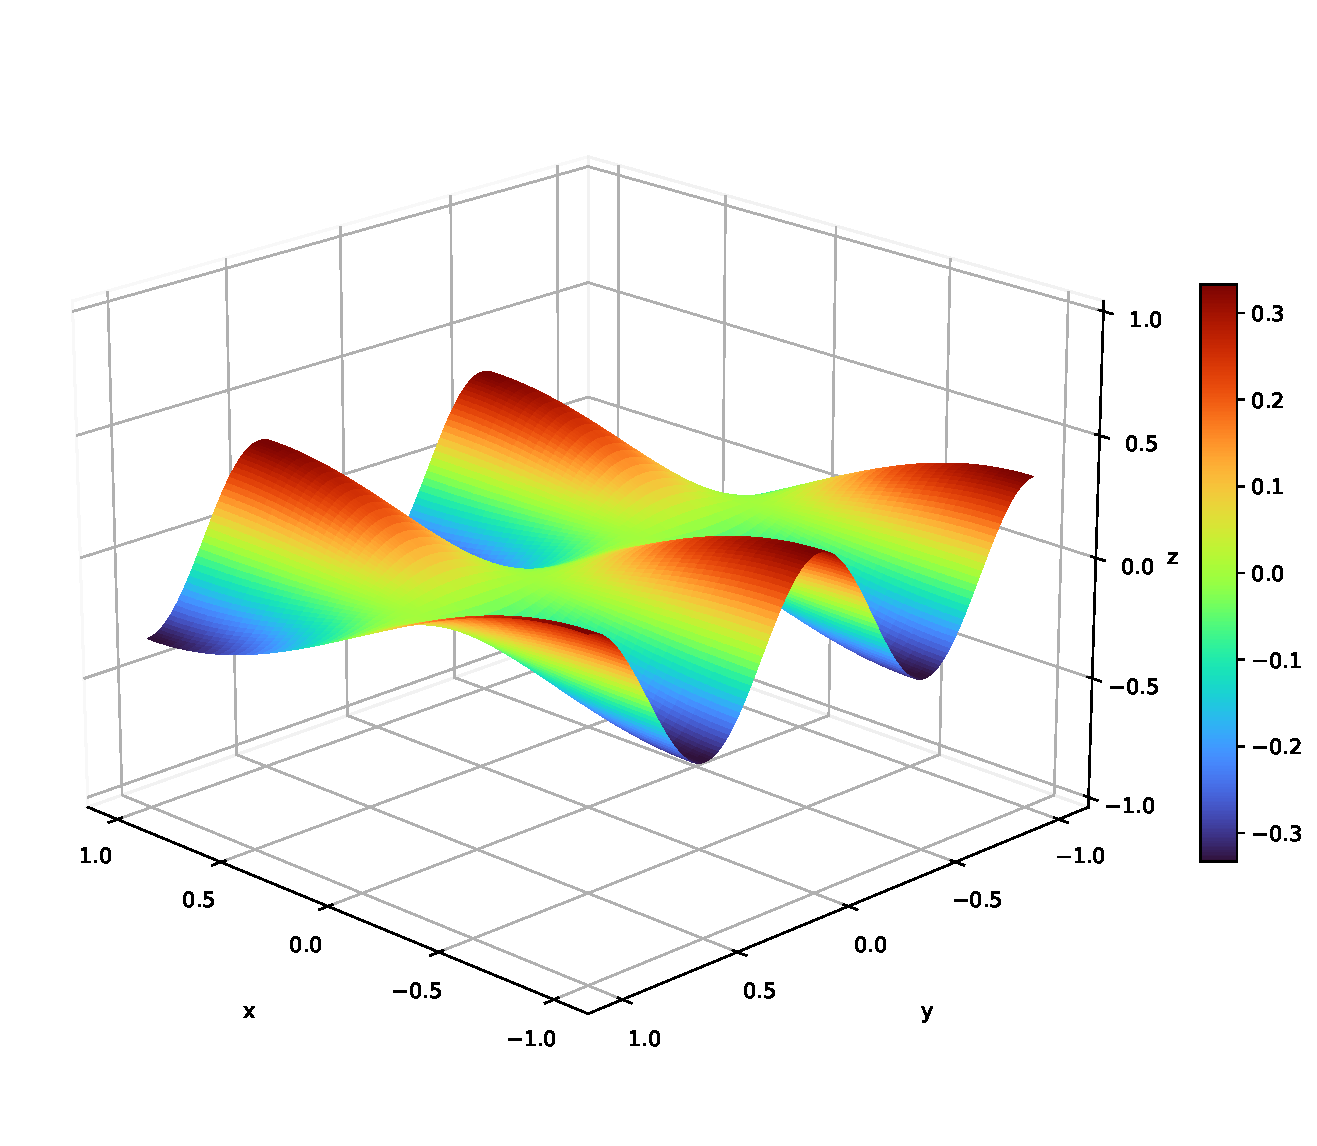
\includegraphics[width=0.5\linewidth]{img/dp_study_analytical.pdf}
  \caption{Analytical solution of the pure Neumann problem}
  \label{fig:dp_neumann_problem_analytical}
\end{figure}




\subsection{Unsteady Stokes Flow}

The review paper \cite{guermond_overview_2006} solves the unsteady Stokes problem

\begin{equation}
  \begin{aligned}
    \bm{u}(\bm{x}, t) &= \pi \sin t 
    \begin{pmatrix}
      \sin( 2\pi y) \sin^2( \pi x) \\
      -\sin(2 \pi x) \sin^2(\pi y)
    \end{pmatrix} \\
    p(\bm{x}, t) &= \sin(t)\cos(\pi x) \sin(\pi y)\\
  \end{aligned}
  \label{eq:MS_stokes_guermond}
\end{equation}
where the source term $f= u_t -\nu \nabla \cdot( \nabla \bm{u} ) + \nabla p $.

In \cite{fehn_stability_2017}, we have
\begin{equation}
  \begin{aligned}
  \bm{u}(\bm{x}, t) &= 
  \begin{pmatrix}
    \sin(x) (a\sin(a y) - \cos(a)\sinh(y)) \\
    \cos(x) (\cos(a y) + \cos(a)\cosh(y))
  \end{pmatrix}
  \exp(-\lambda t),\\
    p(\bm{x}, t) &= \lambda \cos(a) \cos(x) \sinh(y) \exp(-\lambda t)
  \end{aligned}
  \label{eq:MS_unsteady_stokes_fehn}
\end{equation}
where $\lambda = \nu(1 + a^2)$ $\nu = 1$ and $a = 2.883356$ on a domain of  $\Omega = [-1, 1]^2$; they take $[0, T] = [0, 0.1]$ and Dirichlet boundary conditions everywhere, $\Gamma = \Gamma_D$.

\subsection{Verification}
Spatial convergence test, temporal convergence test




\subsection{Taylor-Green vortex flow}
Is this the same test case as in Hesthaven?

\subsection{Backward facing step}

\subsection{Lid-driven cavity flow}

\subsection{Lock Exchange?}
\subsection{Lab RTI flow?}
